% !TEX root = ../main.tex

\chapter{Solution Theory} % Main chapter title
\label{theory} % \ref{theory}


This chapter addresses the solution concepts for the problems that needed to be solved in order to realize the project and is structured according to the previously mentioned main components of the project: object detection, coordinate transformation, and robotic arm control. 
 
\section{Object detection}
The first component of the project is the object detection. Its purpose is to detect objects in the workspace and determine their relative coordinates and size in the image as well as their orientation in relation to the table. 

To simplify these problems, we decided to use a top-down view of the workspace. This means that the camera is positioned above the workspace, so that a linear correlation between the image and the table coordinates emerges. At the early stages of project development the training of a custom object detection model was not intended and it was planned to utilize an existing model. The YOLOv3 model, a convolutional neural network that is trained to detect objects in images, was selected due to its wide array of object classes and its high performance.

To detect the orientation of an object relative to the table, we decided to use OpenCV, a python library used in computer vision applications which provides a broad array of functions for image processing. The main idea was to determine the contours of the object by converting the image into the HSV color space and applying different filter. The contours are then used to calculate the main orientation of the object, using principle component analysis. 

\section{Coordinates transformation}

Once knowing the coordinates of the detected object in the image, 
the next step is to transform the objects position vector from the image's coordinate system to the world's coordinate system. This type of transformation is best achieved with the use of a transformation matrix.

% <!-- the next step is to determine the coordinates of the object in the simulation environment so that its position relative to the robot arm can be used. -->

\subsection{Transformation Matrix}

Assuming a current coordinate system $\mathbf{A}$ and a target coordinate system $\mathbf{B}$, the transformation matrix $\mathbf{T}$ can be used to transform a vector $\vec{v}$ from $\mathbf{A}$ to $\mathbf{B}$.
A transformation matrix can be represented as a matrix frame, built from a combination of a rotation matrix, a translation vector, a scaling vector and a perspective projection matrix.

$$
\mathbf{T} = \left[
\begin{array}{ccc|c}
\ast&\ast       &\ast&\ast\\
\ast&\mathbf{R} &\ast&\vec{t}  \\
\ast&\ast       &\ast&\ast\\
\hline
\ast&\mathbf{P} &\ast&\mathbf{S}
\end{array}
\right]
$$
where:  
* $\mathbf{R}$ is the rotation matrix with the dimensions $3\times 3$.  
* $\vec{t}$ is the translation vector with the dimensions $3\times 1$.  
* $\mathbf{P}$ is the perspective projection matrix with the dimensions $1\times 3$.  
* $\mathbf{S}$ is the scale factor with the dimensions $1\times 1$ (for uniform or isotropic scaling).

The rotation matrix for a rotation around any given axis given by the unit vector $\mathbf{\vec{u}(x,y,z)}$ by an angle $\theta$ is given by the following formula:

$$
\mathbf{R} =
\begin{bmatrix}
u_x^2(1-\cos\theta) + \cos\theta & u_xu_y(1-\cos\theta) - u_z\sin\theta & u_xu_z(1-\cos\theta) + u_y\sin\theta \\
u_xu_y(1-\cos\theta) + u_z\sin\theta & u_y^2(1-\cos\theta) + \cos\theta & u_yu_z(1-\cos\theta) - u_x\sin\theta \\
u_xu_z(1-\cos\theta) - u_y\sin\theta & u_yu_z(1-\cos\theta) + u_x\sin\theta & u_z^2(1-\cos\theta) + \cos\theta \\
\end{bmatrix}
$$

If the rotation is performed around the z axis, the rotation matrix can be simplified to the following form:
$$
\mathbf{R} =
\begin{bmatrix}
\cos\theta & -\sin\theta & 0 \\
\sin\theta & \cos\theta & 0 \\
0 & 0 & 1 \\
\end{bmatrix}
$$


The translation vector is the position of the origin from current coordinate system $O_{current}$ 
relative to the target coordinate system $O_{target}$, i.e. the distance between both origins given as a three dimensional vector. 

$$
\vec{t} =
\begin{bmatrix}
x\\
y\\
z\\
\end{bmatrix}=
O_{current}-O_{target}
$$

The perspective projection matrix is not used in this project due to the camera orientation being perpendicular to the surface of intereset, but is included for completeness.

The scaling factor as given in the frame above can only be used for isotropic scaling, i.e. scaling in all three dimensions by the same factor. Since we are mainly interested in scaling in the x and y directions by different amounts, a single scaling factor can not be used by itself and needs to be expanded to a scaling matrix $\mathbf{S}$ with the following form:

$$
\mathbf{S}=
\begin{bmatrix}
S_x & 0 & 0   & 0\\
0 & S_y & 0   & 0\\
0 & 0   & S_z & 0\\
0 & 0   & 0   & 1
\end{bmatrix}
$$


where $S_x$, $S_y$ and $S_z$ are the scaling factors in the x, y and z directions respectively.

With the rotation and translation matrices a primary Transformation matrix $\mathbf{T_{0}}$ is built with the previously described frame using the unit 1 as a scaling factor and a null matrix as the perspective matrix. 
This is then multiplied with the scaling matrix $\mathbf{S}$ to obtain the complete transformation matrix $\mathbf{T}$ as follows. 

$$\mathbf{T} =  \mathbf{S} \bullet  \mathbf{T_{0}}$$

% <!-- 
% \textcolor{red}{ The following is not complete, needs to be reworked and checked } % end red

% This is done by dividing the dimensions of the table in the simulation by the dimensions of the table in the image. Knowing this, it is possible to generate a transformation matrix

% The first step is to determine the dimensions of the table in order to calculate the scale factor between the image and the simulation. Knowing the scale factor, it is necessary to determine the position and orientation of the table, in order to complete the transformation matrix that needs to be use to calculate the coordinates of the object in the simulation.

% A transformation matrix is a 4x4 matrix that is used to transform a vector from one coordinate system to another. The transformation matrix is calculated by multiplying the translation matrix, the rotation matrix, and the scale matrix. The translation matrix is used to translate the vector from the origin of the coordinate system to the desired position. The rotation matrix is used to rotate the vector around the origin of the coordinate system. The scale matrix is used to scale the vector to the desired size.



% In order to tranform the coordinates from the unit \(pixels\) to the unit \(meters\), the scale matrix is calculated as follows:

% $$
% \begin{bmatrix}
%  width & 0 & 0 & 0 \\
%  0 & height & 0 & 0 \\
%  0 & 0 & depth & 0 \\
%  0 & 0 & 0 & 1 \\
% \end{bmatrix}
% $$

% where \(width\), \(height\), and \(depth\) are the dimensions of the table in the simulation. -->

\section{Robot controller}

The robot controller is the main program where the behaviour of the robot is defined. It is responsible for the different actions that take place in the simulation. By marking the crobot as a supervisor in webots, it can access and modify the properties of other elements in the scene and the environment. 

The main tasks of the robot controller are the following:

\begin{itemize}
    \item Initialization of the different modules and devices
    \item calling of the image processing and object detection modules
    \item performing the required movements of the robotic arm
    \item controlling the movement of the gripper and its fingers
    \item coordinating the actions of the different modules
\end{itemize}

% <!-- 
% It manages and accesses the robot's motors and sensors, and by using the supervisor class from the webots API, it can also have access to the other devices and elements in the simulation. This class allows it to modify the simulation environment and the nodes that are present in the scene, It also provides the capability of accessing and modifying the properties of other elements in the simulation, as well as controlling how the simulation is run.

%  that controlls the robotic arm and accesses the different modules and devices in the simulation. The webots environment provides a supervisor class which provides the capability of accessing and modifyng the properties of other elements in the simulation, as well as controlling how the simulation is run. -->


% <!-- is responsible for the different actions that take place in the simulation. It manages and accesses the robot's motors and sensors of the actions and the access to the other devices in the simulation. It 

% Additionally, a robot-controller needs to be developed to control the robotic arm and the gripper.

% \begin{itemize}
%     \item TODO: first / theoretical approach to solve problem(s)
% \end{itemize}  
% These components will then be integrated into a single routine to detect objects, maneuver the robotic arm to the objects, and relocate the objects to a specified location. -->

\subsection{Robot Kinematics}


The Robot chosen for this task consists of a robotic arm with a gripper attached to the end of the arm. The robot by itself can be represented as a kinematic chain with 6 joints, resulting in 6 degrees of freedom.
In order to move the robot, the target angle of each individual joint in the kinematic chain needs to be set. Nevertheless, the position of the objects and target locations for the robot's movement are defined in a three dimensional coordinate system, so a transformation between the joint angles and the position of the end effector (last chain element) in space needs to be achieved in order to control its movements.

Calculating the position of the gripper (the end effector) from the known position of the individual motor can be achieved using a process called forward kinematics, which combines multiple applications of trigonometric formulas.

Nonetheless, the reverse operation, which aims to calculate the required position of the joints in the kinematic chain for a given position of the end effector presents a more challenging problem. 
This process called inverse kinematics (IK), for which different methods can be used. These methods can be divided into two categories: analytical and numerical.

\begin{figure}[!h]
    \centering
    \includegraphics[width=0.5\textwidth]{Figures/fk_vs_ik.png}
    \caption{Forward and inverse kinematics shown with the green and red arrows respectively.}
    \label{fig:fkik}
\end{figure}

The analytical methods are based on the use of trigonometric formulas, which can be used to calculate the required position values for the motors. However, these methods are limited to a specific number of degrees of freedom, and can only be used for a limited number of cases.

The numerical methods are based on the use of iterative algorithms, which can be used to calculate the required position values for the motors. However, while these methods are not limited to a specific number of degrees of freedom, they can be computationally expensive and are non-deterministic procedures, meaning there can be more than one solution for a given point. Likewise, the time required to find a solution is also non-deterministic, which poses a problem when critical computations need to be performed in real time.


\subsection{Gripper Actuation}

The gripper consists of three individual fingers, each of them having three joints. The closing action of the finger is achieved by rotating the first joint of each finger until the desired object is grabed or the maximum joint rotation is reached. This alone creates a claw like grip, since all finger sections rotate with the first joint relative to the global coordinates. While useful in some cases, its contact area with the object being grabbed is significantly reduced.

A different approach that aims to improve the contact area of the gripper, is possible rotate the last joint of each finger in the opposite direction by the same amount as the first one, compensating the rotation on the fingertips and creating a more stable grip.

The following figure shows the gripper in the open and closed position using the a claw and a pinch grip respectively.

% \begin{figure}[!h]
%     \centering
%     \includegraphics[width=0.5\textwidth]{Figures/red_color.jpg}
%     \caption{From left to rigth: Gripper in open, closed claw, and closed flat positions.}
%     \label{fig:gripper_states}
% \end{figure}

\begin{figure}[!h]
    \centering
    \begin{subfigure}[b]{0.5\textwidth}
        \adjincludegraphics[width=\textwidth]{Figures/grip_open.png}   
        \caption{Open Grip}
    \end{subfigure}\\\vspace{0.5cm}
    
    \begin{subfigure}[b]{0.4\textwidth}
        \adjincludegraphics[width=\textwidth]{Figures/grip_claw.png}        
        \caption{Claw Grip}
    \end{subfigure}
    \hfill
    \begin{subfigure}[b]{0.4\textwidth}
        \adjincludegraphics[width=\textwidth]{Figures/grip_flat.png}        
        \caption{Flat Grip}
    \end{subfigure}\\\vspace{0.5cm}

    \caption{Comparison between the open (resting) position of the gripper with the closed claw and flat grip methods.}
    \label{fig:grip_states}
\end{figure}

\subsection{Movement coordination}

The main loop of actions that need to be taken to complete the task of organizing the desk can be defined as seen in figure ASD. 

The process starts by moving the robot to a HOME position where it wont interfere with the camera's view of the desk. A picture is taken and any objects present are detected. If objects were detected, the robot iterates through the found objects, picking them up and placing them on the a second table on their corresponding position, until all the detected objects have been moved. The robot then moves back to the HOME position. If no object is detected, no movement of the robot takes place. This process is repeated until the user decides to stop the simulation.

% \begin{lstlisting}[]%language=plantuml
% @startuml
% :**Simulation Start**;
% repeat :Move Robot to HOME Position;
%     repeat :Take Picture;
%         :Perform Object Detection;
%     repeat while (objects found?) is (no) not (yes)

%     repeat :Coordinate Transformation;
%         :Move object;
%         :Remove from found objects;
%     repeat while (more objects?) is (yes)
% repeat while (Keep Watching?) is (yes)
% :stop;
% @enduml
% \end{lstlisting}

\begin{figure}[!h]
    \centering
    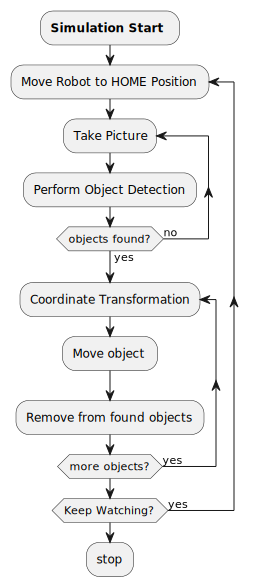
\includegraphics[width=0.5\textwidth]{Figures/sim_loop.png}
    \caption{Flowchart of the main loop of actions}
    \label{fig:flowchart}
\end{figure}

\textcolor{orange}{
. moves to pick up the object and places  
Being able to detect the objects position and orientation, and moving 
With the information regarding the objects' position and orientation in the simulation, the following step is to control the robots movement to produce the desired behavior. The robot controller is implemented in Python and uses the Webots API to control the robot. The robot controller is responsible for the following tasks:
}

\textcolor{orange}{
Initialization of the robot instance and the devices attached to it: 
* camera
* gripper
* internal variables
* Motor sensors
* Motor actuators
}

\textcolor{orange}{
Coordination of the robot's movement.
Coornidation of the different steps required for the organization process.
* Reding the camera's image and forwarding the data to the object detection module.
* Reading the object detection module's output and forwarding the data to the coordinate transformation module.
* Reading the coordinate transformation module's output and forwarding the data to the robotic arm control module.
* Perform the movement as required for the detected objects positions
} %end orange

